% This is samplepaper.tex, a sample chapter demonstrating the
% LLNCS macro package for Springer Computer Science proceedings;
% Version 2.20 of 2017/10/04
%
\documentclass[runningheads]{llncs}
%
\usepackage{graphicx}
\usepackage{color}
\usepackage{amsmath}
\usepackage{amsfonts}
\usepackage{amssymb}
% Used for displaying a sample figure. If possible, figure files should
% be included in EPS format.
%
% If you use the hyperref package, please uncomment the following line
% to display URLs in blue roman font according to Springer's eBook style:
% \renewcommand\UrlFont{\color{blue}\rmfamily}

\setlength{\parindent}{0pt}
\renewcommand{\indent}{\hspace*{0pt}}

\newcommand{\tab}{\hspace*{5mm}}
\newcommand{\qtab}{\hspace*{5mm} \ \quad}

\newcommand{\sif}[3]{\text{if } #1 \text{ then } #2 \text{ else } #3}
\newcommand{\product}[2]{#1 \ prod \ #2}
\newcommand{\tuple}[2]{(#1 :: #2)}
\newcommand{\rearrS}[2]{rearrS \ #1 \ #2}
\newcommand{\rearrV}[2]{rearrV \ #1 \ #2}
\newcommand{\casebx}[6]{case [#1][#2] \to #3, [#4][#5] \to #6}

\newcommand{\bxput}[3]{put \, [\![#1]\!] \ #2 \ #3}
\newcommand{\bxputinline}[1]{put \, [\![#1]\!]}
\newcommand{\bxget}[2]{get \, [\![#1]\!] \ #2}
\newcommand{\bxgetinline}[1]{get \, [\![#1]\!]}

\newcommand{\revput}[3]{put$_{REV}$ \ {#1} \ {#2} \ {#3}}
\newcommand{\revget}[2]{get$_{REV}$ \ {#1} \ {#2}}

\newcommand{\pg}[3]{pg \, [\![#1]\!] (#2, #3)}
\newcommand{\pginline}[1]{pg \, [\![#1]\!]}

\newcommand{\cpg}[5]{cpg [\![#1]\!] (#2, #3, #4, #5)}
\newcommand{\cpginline}[1]{cpg \, [\![#1]\!]}

\newcommand{\kpg}[7]{kpg [\![#1]\!] (#2, #3, #4, #5, #6, #7)}
\newcommand{\kpginline}[1]{kpg \, [\![#1]\!]}

\newcommand{\xpg}[3]{xpg \, [\![#1]\!] (#2, #3)}
\newcommand{\xpginline}[1]{xpg \, [\![#1]\!]}

\begin{document}
%
\title{Bx to Rev (tentative) \thanks{Supported by organization x.}}
%
%\titlerunning{Abbreviated paper title}
% If the paper title is too long for the running head, you can set
% an abbreviated paper title here
%
\author{First Author\inst{1}\orcidID{0000-1111-2222-3333} \and
Second Author\inst{2,3}\orcidID{1111-2222-3333-4444} \and
Third Author\inst{3}\orcidID{2222--3333-4444-5555}}
%
\authorrunning{F. Author et al.}
% First names are abbreviated in the running head.
% If there are more than two authors, 'et al.' is used.
%
\institute{Princeton University, Princeton NJ 08544, USA \and
Springer Heidelberg, Tiergartenstr. 17, 69121 Heidelberg, Germany
\email{lncs@springer.com}\\
\url{http://www.springer.com/gp/computer-science/lncs} \and
ABC Institute, Rupert-Karls-University Heidelberg, Heidelberg, Germany\\
\email{\{abc,lncs\}@uni-heidelberg.de}}
%
\maketitle              % typeset the header of the contribution
%
\begin{abstract}
The abstract should briefly summarize the contents of the paper in
15--250 words.

\keywords{First keyword  \and Second keyword \and Another keyword.}
\end{abstract}
%
%
%
\section{Introduction}

% Story ->
% reversible is needed not to lose any information -> pg is introduced.
% pg is not good for lassoc -> cpg (xpg2) is introduced.
% cpg can be improved -> kpg(xpg) is introduced.
% kpg is slower than pg for rassoc. combined version -> xpg.

% Evaluation result: Comparison with OCaml implementation of miniBiGUL

\begin{itemize}
\item Importance of BX, BX is a solution of view update problem in database.
\item Explanation of put-based BX: BiGUL.
\item Current status of BiGUL: Fastest BX language in the world
\item A problem: Efficiency of compose evaluation. If we do not save the intermediate states, the number of get is quadratic. This is not good.
\item To solve this problem we use an idea from reversible computation: not to lose any information.
\item Based on this idea we introduce pg.
\item We extend pg with several ideas and produce faster implementation.
\end{itemize}

\subsection{Contribution}

\begin{itemize}
\item Improvement of evaluation efficiency
\item Reveal a part of relationship between BX and Reversible.
  \begin{itemize}
  \item Very well-behaved (no adaptive-case) \& The same evaluation path $\to$ No garbage Reversible Computation.
  \item A pair of put and get is self-inverse (involution).
  \item If we can obtain good parameter (dummy) for a BiGUL program,
    put(s, dummy) can be a complement function.
  \end {itemize}
\item Introduced extentions (maybe) use more memory than the original approach, but they are faster than the original.
\end{itemize}

\subsection{Construction of this paper}

\begin{itemize}
\item 
\end{itemize}

\section{Bidirectional Programming Language: BiGUL}

\begin{itemize}
\item our target language is miniBiGUL (BiGUL minus adaptive case) : very well-behaved
\item get = s $\to$ v
\item put = s * v $\to$ s
\item explanation about get and put.
\item We assume putget and getput hold (explanation about putget and getput)
\item explanation about put-based BX language: BiGUL
\item Because our target language satisfies very well-behaved (No adaptive case) $\to$ putput hold.
\end{itemize}

\subsection{Semantics of miniBiGUL}

$\bxput{Skip \ h}{s}{v} = \sif{h \ s = v}{s}{\text{fail}}$

$\bxput{Replace}{s}{v} = v$

$\bxput{\product{bx_1}{bx_2}}{\tuple{s_1}{s_2}}{\tuple{v_1}{v_2}} =\\
    \tab \product{(\bxput{bx_1}{s_1}{v_1})}{(\bxput{bx_2}{s_2}{v_2})}$

$\bxput{\rearrS{f}{bx}}{s}{v} = f^{-1}(\bxput{bx}{(f \ s)}{v})$

$\bxput{\rearrV{g}{bx}}{s}{v} = \bxput{bx}{s}{(g \ v)}$

$\bxput{\casebx{cond_{sv1}}{cond_{s1}}{bx_1}{cond_{sv2}}{cond_{s2}}{bx_2}}{s}{v} = \\
    \tab \text{if } {cond_{sv1} \ s \ v} \\
    \tab \text{then let } s' = \bxput{bx_1}{s}{v} \\
    \tab \text{else let } s' = \bxput{bx_2}{s}{v} \\
    \tab \text{fi } cond_{s1} \ s'; \text{ return } s'$

$\bxput{(bx_1 \circ bx_2)}{s}{v} = \bxput{bx_1}{s}{(\bxput{bx_2}{(\bxget{bx_1}{s})}{v})}$

\vspace{5mm}

$\bxget{Skip \ h}{s} = h \ s$

$\bxget{Replace}{s} = s$

$\bxget{\product{bx_1}{bx_2}}{\tuple{s_1}{s_2}} = \\
    \tab \product{(\bxget{bx_1}{s_1})}{(\bxget{bx_2}{s_2})}$

$\bxget{\rearrS{f}{bx}}{s} = \bxget{bx}{(f \ s)}$

$\bxget{\rearrV{g}{bx}}{s} = g^{-1} (\bxget{bx}{s})$

$\bxget{\casebx{cond_{sv1}}{cond_{s1}}{bx_1}{cond_{sv2}}{cond_{s2}}{bx_2}}{s} =\\
    \tab \text{if } {cond_{s1} \ s}\\
    \tab \text{then let } v' = \bxget{bx_1}{s}\\
    \tab \text{else let } v' = \bxget{bx_2}{s}\\
    \tab \text{fi } {cond_{sv1} \ s \ v'}; \text{ return } v'$

$\bxget{bx_1 \circ bx_2}{s} = \bxget{bx_2}{(\bxget{bx_1}{s})}$

\begin{itemize}
\item To implement this in OCaml, we need some way to produce inverse function for $f$ and $g$.
\item Avoiding this, our implementation requires users to write inverse function f$^{-1}$ and g$^{-1}$.
\end{itemize}

\section{Skip:Reversible langauge: Rwhile}

% Maybe we should skip

\begin{itemize}
\item Usually programs receives inputs and produces outputs. It is impossible to produce inputs from outputs in general. Obtaining the inverse program of a program is difficult.
\item Using reversible language, we can obtain inverse programs easily.
\item Explanation of Rwhile: we need fi-condition.
\item syntax, how to work.
\end{itemize}

\section{Skip:First approach}

% We should skip this 

\begin{itemize}
\item Make put and get to be reversible. We need garbages (g) to keep lost infomation after evaluation.
\item put$_{REV}$ = s * v $\to$ s * g
\item get$_{REV}$ = s $\to$ v * g
\item introduce (put$_{REV}^{-1}$: s * g $\to$ s * v) and (get$_{REV}^{-1}$:v * g $\to$ s)
\item \textcolor{red}{(Missing part?)} Relationship between put$_{REV}$, get$_{REV}$, put$_{REV}^{-1}$, get$_{REV}^{-1}$ 
\end{itemize}




% \noindent
% \revput{(Skip $h$)}{s}{v} = \sif{$h$ s = v}{(s, v)}{fail}

% \noindent
% \revput{Replace}{s}{v} = (v, s)

% \noindent
% \revput{\product{$bx_1$}{$bx_2$}}{\tuple{$s_1$}{$s_2$}}{\tuple{$v_1$}{$v_2$}} =\\
% \hspace{5mm}let (s1, g1) = \revput{$bx_1$}{$s_1$}{$v_1$} in\\
% \hspace{5mm}let (s2, g2) = \revput{$bx_2$}{$s_2$}{$v_2$} in\\
% \hspace{5mm}((s1, s2), (g1, g2))

% \noindent
% \revput{(\rearrS{$f$}{bx})}{s}{v} =\\
% \hspace{5mm}let (s1, g1) = \revput{bx}{($f$ s)}{v} in\\
% \hspace{5mm}($f^{-1}$ s1, g1)

% \noindent
% \revput{(\rearrV{$g$}{bx})}{s}{v} =\\
% \hspace{5mm} let (s1, g1) = \revput{bx}{s}{($g$ v)} in\\
% \hspace{5mm} (s1, g1)

% \noindent
% \revput{(\casebx{cond$_{sv1}$}{cond$_{s1}$}{bx$_1$}{cond$_{sv2}$}{cond$_{s2}$}{bx$_2$})}{s}{v} =\\
% \hspace{5mm} if {cond$_{sv1}$ s v}\\
% \hspace{5mm} then let (s', g) = \revput{bx$_1$}{s}{v} in\\
% \hspace{5mm} else let (s', g) = \revput{bx$_2$}{s}{v} in\\
% \hspace{5mm} fi cond$_{s1}$ s'; return (s', g)

% \noindent
% \revput{(bx$_1$ $\circ$ bx$_2$)}{s}{v} =\\
% \hspace{5mm} let (s1, g1) = \revget{bx$_1$}{s} in\\
% \hspace{5mm} let (s2, g2) = \revput{bx$_2$}{s1}{v} in\\
% \hspace{5mm} let (s3, g3) = \revput{bx$_1$}{s}{s2} in (* need to copy s *)\\
% \hspace{5mm} (s3, (g1, g2, g3))


% \vspace{5mm}
% \noindent
% \revget{(Skip $h$)}{s} = {($h$ s, s)}

% \noindent
% \revget{Replace}{s} = (s, \textcolor{red}{Nil})

% \noindent
% \revget{\product{$bx_1$}{$bx_2$}}{\tuple{$s_1$}{$s_2$}} = \\
% \hspace{5mm} let (v1, g1) = \revget{$bx_1$}{$s_1$} in\\
% \hspace{5mm} let (v2, g2) = \revget{$bx_2$}{$s_2$} in\\
% \hspace{5mm} ((v1, v2), (g1, g2))

% \noindent
% %% from here
% \revget{(\rearrS{$f$}{bx})}{s}{v} =\\
% \hspace{5mm}let (v1, g1) = \revget{bx}{($f$ s)} in\\
% \hspace{5mm}(v1, g1)

% \noindent
% \revget{(\rearrV{$g$}{bx})}{s}{v} =\\
% \hspace{5mm} let (v1, g1) = \revget{bx}{s} in\\
% \hspace{5mm} ($g^{-1}$ v1, g1)

% \noindent
% \revget{(\casebx{cond$_{sv1}$}{cond$_{s1}$}{bx$_1$}{cond$_{sv2}$}{cond$_{s2}$}{bx$_2$})}{s} =\\
% \hspace{5mm} if {cond$_{s1}$ s}\\
% \hspace{5mm} then let (v', g) = \revget{bx$_1$}{s} in\\
% \hspace{5mm} else let (v', g) = \revget{bx$_2$}{s} in\\
% \hspace{5mm} fi cond$_{sv1}$ s v'; return (v', g)

% \noindent
% \revget{(bx$_1$ $\circ$ bx$_2$)}{s}{v} =\\
% \hspace{5mm} let (v1, g1) = \revget{bx$_1$}{s} in\\
% \hspace{5mm} let (v2, g2) = \revget{bx$_1$}{s} in\\
% \hspace{5mm} (v2, (g1, g2))

\textcolor{red}{If we use Rwhile for target language, we do not need to introduce inverse.}

\section{pg}
\subsection{Self-inverse function: pg}

\begin{itemize}
\item Information loss causes re-evaluation of get.
\item To prevent this, we introduced the idea of reversible computation.
\item In reversible computation we need to keep all information: we can not lose any information.
\item In BiGul we can do this with a pair of put and get.
\item pg bx (s, v) = (put bx (s, v), get bx (s))
\item pg: s * v $\to$ s * v
\item No garbage
\item This function is self-inverse. (involution, (f (f input)) = input)
\item \textcolor{red}{Constraint: In case expression, put and get must always choose the same branch. This constraint is not satisfied in general: (e.g, SNOC, the different length of two inputs.) To remove this constraint we need to use garbage.}
\end{itemize}

For the approaches so far, when evaluating a composition of BX programs, $get$s are re-evaluated so many times since no intermediate state is stored during the evaluation. This is a kind of information loss. One question is whether it is possible to calculate the above programs without losing information. And the answer is yes. It comes from the the idea of reversible computation where all information during the evaluation need to be kept. In miniBiGUL, we can do that by tupling $put$ and $get$. The such pair is accepted as input of a function named $pg$ to produce a new one that contains the actual result of a BX program.

\textbf{Definition:} \\
$\pg{bx}{s}{v} = (\bxput{bx}{s}{v}, \bxget{bx}{s})$ \\

$pg$ is an involution that is self-inverse. An involution is a function $f$ that satifies $f(f(x)) = x \text{ for all } x \text{ in the domain of } f$.

Proof:\\
$pg [\![bx]\!] \ (\pg{bx}{s}{v}) \\
    \tab = \pg{bx}{(\bxput{bx}{s}{v})}{(\bxget{bx}{s})} \quad [pg \text{ definition}] \\
    \tab = (put \ [\![bx]\!] \ (\bxput{bx}{s}{v}) \ (\bxget{bx}{s}), \bxget{bx}{(\bxput{bx}{s}{v})})  \quad [pg \text{ definition}] \\
    \tab = (put \ [\![bx]\!] \ (\bxput{bx}{s}{v}, \bxget{bx}{s}), v) \quad [\text{PUTGET}] \\
    \tab = (put \ [\![bx]\!] \ (s, \bxget{bx}{s}), v) \quad [\text{PUTPUT}] \\
    \tab = (s, v) \quad [\text{GETPUT}]$

\subsection{Skip:Construction of pg}

$\pg{Skip \ h}{s}{v} \\
    \tab = (\sif{h \ s = v}{s}{\text{fail}}, h \ s) \\
    \tab = \sif{h \ s = v}{(s, h \ s)}{\text{fail}} \\
    \tab = \sif{h \ s = v}{(s, v)}{\text{fail}}$

There is a trick in the construction of $\pginline{Skip \ h}$. The first equality is simply based on the definitions of $pg$, $\bxputinline{Skip \ h}$ and $\bxgetinline{Skip \ h}$. The second one tuples two results of $put$ and $get$ in the body of the if-expression. And the last one is quite obivious. What we call the trick here is in the second equality where in some cases, the result of $pg$ may be fail although there is no fail when evaluating $\bxgetinline{Skip \ h}$.\\

$\pg{Replace}{s}{v}\\
    \tab = (v, s)$

$\pg{\product{bx_1}{bx_2}}{\tuple{s_1}{s_2}}{\tuple{v_1}{v_2}} \\
    \tab = (\product{(\bxput{bx_1}{s_1}{v_1})}{(\bxput{bx_2}{s_2}{v_2})}, \product{(\bxget{bx_1}{s_1})}{(\bxget{bx_2}{s_2})}) \\
    \tab = \text{let } (s_1, v_1) = \pg{bx_1}{s_1}{v_1} \text{ in} \\
        \qtab \text{let } (s_2, v_2) = \pg{bx_2}{s_2}{v_2} \text{ in} \\
        \qtab (\product{s_1}{s_2}, \product{v_1}{v_2})$

$\pg{\rearrS{f}{bx}}{s}{v} \\
    \tab = (f^{-1}(\bxput{bx}{(f \ s)}{v}), \bxget{bx}{(f \ s)}) \\
    \tab = \text{let } (s, v) = \pg{bx}{(f \ s)}{v} \text{ in} \\
        \qtab (f^{-1} s, v)$

$\pg{\rearrV{g}{bx}}{s}{v} \\
    \tab = (\bxput{bx}{s}{(g v)}, g^{-1} (\bxget{bx}{s})) \\
    \tab = \text{let } (s, v) = \pg{bx}{s}{(g v)} \text{ in} \\
        \qtab (s, g^{-1} v)$\\

Constructions of $pg$ for $[\![Replace]\!]$, $[\![\product{bx_1}{bx_2}]\!]$, $[\![\rearrS{f}{bx}]\!]$ and $[\![\rearrV{g}{bx}]\!]$ are very clear when just paring $put$ and $get$ respectively, then doing basic changes.\\

$\pg{\casebx{cond_{sv1}}{cond_{s1}}{bx_1}{cond_{sv2}}{cond_{s2}}{bx_2}}{s}{v} \\
    \tab = (\text{if } {cond_{sv1} \ s \ v} \\
    \qtab \text{then let } s' = \bxput{bx_1}{s}{v} \\
    \qtab \text{else let } s' = \bxput{bx_2}{s}{v} \\
    \qtab \text{fi } cond_{s1} \ s'; \text{ return } s', \\
    \qtab \quad \text{if } {cond_{s1} \ s}\\
    \qtab \quad \text{then let } v' = \bxget{bx_1}{s}\\
    \qtab \quad \text{else let } v' = \bxget{bx_2}{s}\\
    \qtab \quad \text{fi } {cond_{sv1} \ s \ v'}; \text{ return } v') \\
    \tab = \text{if } {cond_{sv1} \ s \ v} \ and \ {cond_{s1} \ s} \\
        \qtab \text{then let } (s', v') = \pg{bx_1}{s}{v}\\
        \qtab \text{else let } (s', v') = \pg{bx_2}{s}{v}\\
        \qtab \text{fi } cond_{v1} \ s' \ and \ cond_{sv1} \ s \ v'; \text{ return } (s',v')$\\

A restriction for $\pginline{case}$ needs to be introduced here. We know that there is one entering condition and one exit condition when evaluating $\bxputinline{case}$ as well as $\bxgetinline{case}$. If a tupling $put$ and $get$ occurs, there will be 4 combinations of these conditions. This means that two entering conditions of $\bxputinline{case}$ and $\bxgetinline{case}$ are not always simultaneously satified. The evaluated BXs are different in the $put$ and $get$ directions for combinations $((cond_{sv1} \ s \ v) \ and \ (not (cond_{s1} \ s)))$ and $((not (cond_{sv1} \ s \ v) \ and \ (cond_{s1} \ s))$, which are restricted in this paper. This does not happen for the others, which the construction of $\pginline{case}$ uses above. \\


$\pg{bx_1 \circ bx_2}{s}{v} \\
    \hspace*{5mm} = (\bxput{bx_1}{s}{(\bxput{bx_2}{(\bxget{bx_1}{s})}{v})}, \bxget{bx_2}{(\bxget{bx_1}{s})}) \\
    \hspace*{5mm} = \text{let } a = \bxget{bx_1}{s} \text{ in} \\
        \hspace*{5mm} \ \quad \text{let } (b, c) = \pg{bx_2}{a}{v} \text{ in} \\
        \hspace*{5mm} \ \quad \text{let } (d, e) = \pg{bx_1}{s}{b} \text{ in} \\
        \hspace*{5mm} \ \quad (d, c) \\
    \hspace*{5mm} = \text{let } (f, a) = \pg{bx_1}{s}{dummy} \text{ in} \\
        \hspace*{5mm} \ \quad \text{let } (b, c) = \pg{bx_2}{a}{v} \text{ in} \\
        \hspace*{5mm} \ \quad \text{let } (d, e) = \pg{bx_1}{s}{b} \text{ in} \\
        \hspace*{5mm} \ \quad (d, c) \\
    \hspace*{5mm} = \text{let } (f, a) = \pg{bx_1}{s}{dummy} \text{ in} \\
        \hspace*{5mm} \ \quad \text{let } (b, c) = \pg{bx_2}{a}{v} \text{ in} \\
        \hspace*{5mm} \ \quad \text{let } (d, e) = \pg{bx_1}{\textcolor{red}{f}}{b} \text{ in} \\
        \hspace*{5mm} \ \quad (d, c)$\\

The construction of $\pginline{bx_1 \circ bx_2}$ can be considered as the soul of the $pg$ function. The first two equalities comes from mentioned definitions and some basic transformations. The third one rewrites $(\text{let } a = \bxget{bx_1}{s} \text{ in})$ into $(\text{let } (f, a) = \pg{bx_1}{s}{dummy} \text{ in})$. It is possible if we consider $(\bxget{bx_1}{s})$ as the second element of $(\pg{bx_1}{s}{dummy})$ where $dummy$ is a special value that make the $put \, [\![bx_1]\!]$ direction is valid. The last equality substitutes $s$ in $(\text{let } (d, e) = \pg{bx_1}{s}{b} \text{ in})$ by $f$ which is the evaluated result of $\bxput{bx_1}{s}{dummy}$. This transformation is feasible due to the PUTPUT law. Then, $e$ in the result pair $(d,e)$ of the new let-expression equals $dummy$. So we can realize that there is no loss information when computing a composition.

\subsection{How to Evaluate Bidirectional Programs using pg}

\begin{itemize}
\item Because we combine put and get, we need to supply view for evaluation of get.
\item introduce dummy?
\item automatic analysis for domain \& range?
\item 
\item partial evaluation of put(s(D), dummy(S)).
\item \textcolor{red}{Not good? Basically put (BX) is often a recursion on the source. If source is static, partial evaluation will work well. On the other hand, view is small data. So partial evaluation might not work well.}
\item \textcolor{red}{lazy evaluation is also a possibility?}
\end{itemize}

\subsection{cpg}

\begin{itemize}
\item If the BX programs are left assoc of composition, pg will be exponential. Because it calls pg bx$_1$ twice.
\item To solve this problem, we introduce accumulation of changes.
\end{itemize}

$fst = \lambda (Con (x1, x2)). x1$\\
$snd = \lambda (Con (x1, x2)). x2$\\
$con = \lambda ks1. \lambda ks2. \lambda x. Con(ks1 \ x, ks2 \ x)$\\

$\cpg{bx}{ks}{kv}{s}{v}$ \\
    \tab $ks, kv$ evaluate actual values\\
    \tab $s, v$ keep evaluated values\\
\vspace{3mm}

$\cpg{Skip \ h}{ks}{kv}{s}{v} = \text{ if } h \ s = v \text{ then } (ks, kv, s, v) \text{ else fail}$\\

$\cpg{Replace}{ks}{kv}{s}{v} = (kv, ks, v, s)$\\

$\cpg{\product{bx_1}{bx_2}}{ks}{kv}{s}{v} =\\
    \tab (ks1, kv1, s1, v1) \Leftarrow \cpg{bx1}{fst \circ ks}{fst \circ kv}{fst \ s}{fst \ v};\\
    \tab (ks2, kv2, s2, v2) \Leftarrow \cpg{bx2}{snd \circ ks}{snd \circ kv}{snd \ s}{snd \ v};\\
    \qtab ((con \ ks1 \ ks2, con \ kv1 \ kv2, Con \ s1 \ s2, Con \ v1 \ v2)$\\

$\cpg{RearrS \ f1 \ f2 \ bx}{ks}{kv}{s}{v} =\\
    \tab (ks, kv, s, v) \Leftarrow \cpg{bx}{f1 \circ ks}{kv}{f1 \ s}{v};\\
    \qtab (f2 \circ ks, kv, s, v)$\\

$\cpg{RearrV \ g1 \ g2 \ bx}{ks}{kv}{s}{v} =\\
    \tab (ks, kv, s, v) \Leftarrow \cpg{bx}{ks}{g1 \circ kv}{s}{g1 \ v};\\
    \qtab (ks, g2 \circ kv, ks, g2 \ v)$\\

$\cpg{Case \ c \ bx1 \ bx2}{ks}{kv}{s}{v} =\\
    \tab \text{if} \ c \ s \ v \ \text{then}\\
        \qtab \cpg{bx1}{ks}{kv}{s}{v}\\
    \tab \text{else} \\ 
        \qtab \cpg{bx2}{ks}{kv}{s}{v}$\\

$\cpg{bx1 \circ bx2}{ks}{kv}{s}{v} =\\
    \tab (ks1, kv1, \underline{s1}, v1) \Leftarrow \cpg{bx1}{ks}{id}{s}{const$\_$dummy \ v};\\
    \tab (ks2, kv2, s2, v2) \Leftarrow \cpg{bx2}{kv1}{kv}{v1}{v};\\
        \qtab (ks1 \circ ks2, kv2,  ks1 \ s2, v2)$\\

\begin{itemize}
\item This is faster than pg for left assoc BX programs.
\item (Slower for right assoc programs)
\item $s1'$ in composition is redundant.  
\item Next, we will extend this to avoid this redundant computation.
\end{itemize}


\subsection{kpg}

$\kpg{bx}{ks'}{kv'}{ks}{kv}{s}{v}$ \\
    \tab $ks', kv'$ keep modification information\\
    \tab $ks, kv$ evaluate actual values\\
    \tab $s, v$ keep evaluated values\\

$\kpg{Skip \ h}{ks'}{kv'}{ks}{kv}{s}{v} =\\
    \tab s \Leftarrow ks \ s;\\
    \tab v \Leftarrow kv \ v;\\
    \tab \text{if} \ h \ s = v \ \text{then} \ (ks', kv', id, id, s, v) \ \text{else fail}$\\

$\kpg{Replace}{ks'}{kv'}{ks}{kv}{s}{v} = (kv', ks', kv, ks, v, s)$\\

$\kpg{bx1 \ prod \ bx2}{ks'}{kv'}{ks}{kv}{s}{v} =\\
    \textcolor{red}{s \Leftarrow ks \ s; v \Leftarrow kv \ v; ks \Leftarrow id; kv \Leftarrow id;}\\
    (ks1', kv1', ks1, kv1, s1, v1) \Leftarrow \kpg{bx1}{fst \circ ks'}{fst \circ kv'}{fst \circ ks}{fst \circ kv}{s}{v};\\
    (ks2', kv2', ks2, kv2, s2, v2) \Leftarrow \kpg{bx2}{snd \circ ks'}{snd \circ kv'}{snd \circ ks}{snd \circ kv}{s}{v};\\
    \tab ( con \ ks1' \ ks2', con \ kv1' \ kv2', \\
    \qtab con \ (ks1 \circ fst) \ (ks2 \circ snd), con \ (kv1 \circ fst) \ (kv2 \circ snd), \\
    \qtab (Con \ s1 \ s2), (Con \ v1 \ v2))$\\

$\kpg{RearrS \ f1 \ f2 \ bx}{ks'}{kv'}{ks}{kv}{s}{v} =\\
    \tab (ks', kv', ks, kv, s, v) \Leftarrow \kpg{bx}{f1 \circ ks'}{kv'}{f1 \circ ks}{kv}{s}{v};\\
    \qtab (f2 \circ ks', kv', f2 \circ ks, kv, s, v)$\\

$\kpg{RearrV \ g1 \ g2 \ bx}{ks'}{kv'}{ks}{kv}{s}{v} =\\
    \tab (ks', kv', ks, kv, s, v) \Leftarrow \kpg{bx}{ks'}{g1 \circ kv'}{ks}{g1 \circ kv}{s}{v};\\
    \qtab (ks', g2 \circ kv', ks, g2 \circ kv, s, v)$\\

$\kpg{Case \ c \ bx1 \ bx2}{ks'}{kv'}{ks}{kv}{s}{v} =\\
    \tab s \Leftarrow ks \ s;\\
    \tab v \Leftarrow kv \ v;\\
    \tab \text{if} \ c \ s \ v \ \text{then}\\
        \qtab \kpg{bx1}{ks'}{kv'}{id}{id}{s}{v}\\
    \tab \text{else}\\\
        \qtab \kpg{bx2}{ks'}{kv'}{id}{id}{s}{v}$\\

$\kpg{bx1 \circ bx2}{ks'}{kv'}{ks}{kv}{s}{v} =\\
    \tab (ks1', kv1', \underline{ks1}, kv1, \underline{s1}, v1) \Leftarrow \kpg{bx1}{ks'}{id}{ks}{id}{s}{const$\_$dummy \ v};\\
    \tab (ks2', kv2', ks2, kv2, s2, v2) \Leftarrow \kpg{bx2}{kv1'}{kv'}{kv1}{kv}{v1}{v};\\
    \qtab (ks1' \circ ks2', kv2', ks1' \circ ks2, kv2, s2, v2)$

\begin{itemize}
\item In this definition of kpg, s' and v' will have actual value only in skip and case. Except them, the functions for computation will be kept as ks' and kv'.
\item In composition $ks1'$ and $s1'$ are still redundant. But, they are not evaluated.
\item In prod, Evaluation of ks' and kv' will be done indendently in kpg$[\![bx_1]\!]$ and kpg$[\![bx_2]\!]$. To remove redundant re-computation we evaluate actual s' and v'.
\item This implementation is faster for left assoc BX programs. (Actually slower for right assoc than cpg)
\end{itemize}

\section{xpg}

\begin{itemize}
\item pg is fastest for right assoc programs and kpg is fastest for left assoc programs.
\item To combine their strength, we can use the following definition.
\item If there is a composition, we use xpg for evaluation of $bx_1$ and pg for evaluation of $bx_2$.
\item If $bx_1$ is simple program (= Right assoc), this is almost the same with pg.
\item If $bx_1$ is complicated program (= Left assoc), this is almost the same with kpg.
\end{itemize}

$\xpg{E}{s}{v} = \text{same with } pg \text{ if } E \text{ is not compose}$

$\xpg{bx_1 \circ bx_2}{s}{v} =\\
    \tab (ks1',kv1', ks1, kv1, s1, v1) \Leftarrow \kpg{bx_1}{id}{id}{\lambda \_.s}{id}{s}{v};\\
    \tab (s2, v2) \Leftarrow \xpg{bx_2}{kv1 \ v1}{v};\\
    \qtab (ks1' \ s2, v2)$

\section{Experimental result}

\begin{itemize}
\item Evaluation time for miniBiGul, pg, cpg, kpg, xpg.
\item Memory allocation of miniBiGul, pg, cpg, kpg, xpg.
\item []
\item xpg looks the best one (maybe)
\item 
\end{itemize}

\subsection{Theoretical Computational Complexity}

\section{Conclusion and Future Work}


% From sample code
% 
% ---- Bibliography ----
%
% BibTeX users should specify bibliography style 'splncs04'.
% References will then be sorted and formatted in the correct style.
%
% \bibliographystyle{splncs04}
% \bibliography{mybibliography}
%
\begin{thebibliography}{8}
\bibitem{ref_article1}
Author, F.: Article title. Journal \textbf{2}(5), 99--110 (2016)

\bibitem{ref_lncs1}
Author, F., Author, S.: Title of a proceedings paper. In: Editor,
F., Editor, S. (eds.) CONFERENCE 2016, LNCS, vol. 9999, pp. 1--13.
Springer, Heidelberg (2016). \doi{10.10007/1234567890}

\bibitem{ref_book1}
Author, F., Author, S., Author, T.: Book title. 2nd edn. Publisher,
Location (1999)

\bibitem{ref_proc1}
Author, A.-B.: Contribution title. In: 9th International Proceedings
on Proceedings, pp. 1--2. Publisher, Location (2010)

\bibitem{ref_url1}
LNCS Homepage, \url{http://www.springer.com/lncs}. Last accessed 4
Oct 2017
\end{thebibliography}
\end{document}







\subsubsection{Sample Heading (Third Level)} Only two levels of
headings should be numbered. Lower level headings remain unnumbered;
they are formatted as run-in headings.

\paragraph{Sample Heading (Fourth Level)}
The contribution should contain no more than four levels of
headings. Table~\ref{tab1} gives a summary of all heading levels.

\begin{table}
\caption{Table captions should be placed above the
tables.}\label{tab1}
\begin{tabular}{|l|l|l|}
\hline
Heading level &  Example & Font size and style\\
\hline
Title (centered) &  {\Large\bfseries Lecture Notes} & 14 point, bold\\
1st-level heading &  {\large\bfseries 1 Introduction} & 12 point, bold\\
2nd-level heading & {\bfseries 2.1 Printing Area} & 10 point, bold\\
3rd-level heading & {\bfseries Run-in Heading in Bold.} Text follows & 10 point, bold\\
4th-level heading & {\itshape Lowest Level Heading.} Text follows & 10 point, italic\\
\hline
\end{tabular}
\end{table}


\noindent Displayed equations are centered and set on a separate
line.
\begin{equation}
x + y = z
\end{equation}
Please try to avoid rasterized images for line-art diagrams and
schemas. Whenever possible, use vector graphics instead (see
Fig.~\ref{fig1}).

\begin{figure}
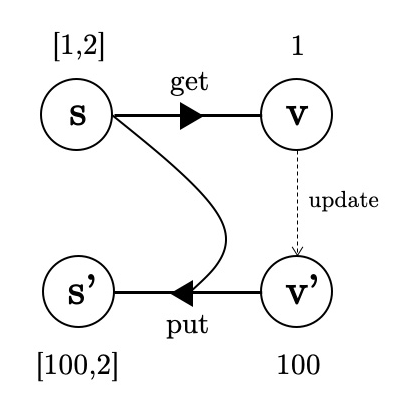
\includegraphics[width=\textwidth]{fig1.eps}
\caption{A figure caption is always placed below the illustration.
Please note that short captions are centered, while long ones are
justified by the macro package automatically.} \label{fig1}
\end{figure}

\begin{theorem}
This is a sample theorem. The run-in heading is set in bold, while
the following text appears in italics. Definitions, lemmas,
propositions, and corollaries are styled the same way.
\end{theorem}
%
% the environments 'definition', 'lemma', 'proposition', 'corollary',
% 'remark', and 'example' are defined in the LLNCS documentclass as well.
%
\begin{proof}
Proofs, examples, and remarks have the initial word in italics,
while the following text appears in normal font.
\end{proof}
For citations of references, we prefer the use of square brackets
and consecutive numbers. Citations using labels or the author/year
convention are also acceptable. The following bibliography provides
a sample reference list with entries for journal
articles~\cite{ref_article1}, an LNCS chapter~\cite{ref_lncs1}, a
book~\cite{ref_book1}, proceedings without editors~\cite{ref_proc1},
and a homepage~\cite{ref_url1}. Multiple citations are grouped
\cite{ref_article1,ref_lncs1,ref_book1},
\cite{ref_article1,ref_book1,ref_proc1,ref_url1}.
%
